\documentclass[10pt]{article}

\usepackage{amssymb,amsmath}
\usepackage{graphicx}
\usepackage[hidelinks]{hyperref}
\usepackage[a4paper, left=2cm, right=2cm, top=2.5cm, bottom=2.5cm]{geometry}
\usepackage{float}
\usepackage{caption}

\title{Reinforcement Learning Project\\
\large Reward Misspecification and Its Impact on Learning Dynamics}

\author{Victor Schmit}
\date{\today}

\begin{document}

\maketitle

\begin{abstract}
	Reinforcement learning (RL) agents optimize the reward signal they receive from the environment, which makes reward design a central component of the learning process. In this project, we study how different reward formulations affect learning dynamics, value estimation, policy structure, and robustness in a tabular RL setting. We consider a stochastic gridworld environment and compare two classical agents, Q-learning and SARSA, under three reward schemes: a correctly specified reward, a misspecified reward introducing a misleading incentive, and a potential-based shaping reward. The experiments show that reward misspecification can induce reward hacking, with agents obtaining high return while failing to solve the intended task. In contrast, potential-based reward shaping accelerates learning while preserving the optimal policy. Overall, the study highlights that reward specification can have a stronger impact on behavior than the choice of learning algorithm itself.
\end{abstract}

\tableofcontents
\newpage

\section{Introduction}

Reinforcement Learning (RL) provides a framework for sequential decision-making in which an agent learns through trial and error by interacting with an environment. At each time step, the agent observes a state, takes an action, and receives a reward. The objective is to maximize the expected cumulative reward over time. This paradigm is powerful because it avoids direct supervision and instead relies on a scalar feedback signal.

However, this also makes RL particularly sensitive to the design of the reward function. In theory, the reward should encode the true objective of the task. In practice, it is often only an imperfect proxy. When this happens, the agent may discover behaviors that maximize reward without actually solving the intended problem. This phenomenon is commonly referred to as \emph{reward misspecification} or \emph{reward hacking}.

A second challenge is that even a correctly specified reward may be difficult to learn from if it is too sparse. This motivates the use of reward shaping, that is, additional signals designed to guide the agent during learning. Yet such modifications are delicate: they can either improve sample efficiency or alter the underlying optimization target.

The aim of this project is therefore twofold. First, we analyze how different reward formulations modify the learning behavior of tabular RL agents. Second, we study whether principled reward shaping can improve learning speed while preserving the intended objective.

\section{Algorithms}

We consider two standard tabular reinforcement learning algorithms: Q-learning and SARSA. Both learn an estimate of the action-value function $Q(s,a)$, but they differ in the way future rewards are propagated backward.

Q-learning is an off-policy method. Its update rule is
\[
	Q(s,a) \leftarrow Q(s,a) + \alpha \bigl(r + \gamma \max_{a'} Q(s',a') - Q(s,a)\bigr),
\]
where $\alpha$ is the learning rate and $\gamma$ the discount factor. The use of the maximum over next actions makes Q-learning optimistic: it updates toward the value of the best possible future action, independently of the behavior policy currently used for exploration. In practice, this often leads to faster learning, but it also makes Q-learning more sensitive to reward bias, since overestimated rewards can be propagated aggressively.

SARSA is an on-policy method. Its update rule is
\[
	Q(s,a) \leftarrow Q(s,a) + \alpha \bigl(r + \gamma Q(s',a') - Q(s,a)\bigr),
\]
where $a'$ is the next action actually selected by the current behavior policy. Unlike Q-learning, SARSA incorporates exploration and stochasticity directly into its updates. This makes it more conservative, particularly in environments with risk or action noise, and therefore often more robust but slower to converge.

We compare both algorithms under the same experimental conditions to verify that the observed effects are genuinely related to reward design and not only to the update rule.

\section{Environment}

We consider a gridworld environment modeled as a Markov Decision Process $(\mathcal{S}, \mathcal{A}, P, R, \gamma)$. The state space consists of positions on a finite grid, and the action space is given by the four cardinal moves:
\[
	\mathcal{A} = \{\text{up}, \text{down}, \text{left}, \text{right}\}.
\]

The environment contains a start state, a goal state, obstacles, and a cliff region. Entering the cliff leads to a strong penalty and resets the agent to the start. The environment is also stochastic: with a fixed probability, the intended action is not executed exactly, introducing slippage in the transitions. This makes the task more difficult and increases the importance of robust decision-making.

Compared with a minimal gridworld, the environment was made more challenging by introducing multiple admissible paths and risky shortcut regions. This prevents the task from degenerating into a trivial shortest-path problem and makes it possible to observe how reward specification shapes behavior in a non-trivial way.

\section{Reward Specification}

A central aspect of the project is the comparison of three reward formulations.

The first one is the \textbf{correct reward}, designed to align directly with the intended task: reaching the goal efficiently while avoiding dangerous states. In practice, this means a positive reward for the goal, a small step penalty to encourage short paths, and a strong penalty for cliff states.

The second one is a \textbf{misspecified reward}. In this setting, an additional positive incentive is introduced in a lure region located near the cliff. Although this modification appears to provide a denser signal, it creates a misleading objective: the agent can accumulate reward in this region without solving the task.

The third formulation is \textbf{potential-based reward shaping}, defined by
\[
	R'(s,a,s') = R(s,a,s') + \gamma \Phi(s') - \Phi(s),
\]
where $\Phi(s)$ is a potential function. In our case, $\Phi(s)$ is chosen as the negative Manhattan distance to the goal. This transformation is theoretically important because it preserves the optimal policy while providing a denser learning signal. Unlike naive shaping, it improves learning efficiency without changing what the agent should ultimately do.

\section{Experimental Protocol}

All agents are trained using an $\varepsilon$-greedy exploration policy with a decaying exploration rate. The learning rate, discount factor, and other training hyperparameters are kept fixed across experiments in order to isolate the effect of reward design.

For each configuration, we record multiple complementary metrics:
\begin{itemize}
	\item the cumulative reward per episode,
	\item the success rate, defined as the proportion of episodes reaching the goal,
	\item the learned policy,
	\item the estimated value function,
	\item state visitation frequencies,
	\item and representative greedy trajectories.
\end{itemize}

This combination of quantitative and qualitative diagnostics is essential. A single scalar metric such as return can be misleading, especially when misspecified rewards allow the agent to accumulate reward without achieving the intended objective.

\section{Results}

\subsection{Learning curves and success rates}

\begin{figure}[H]
	\centering
	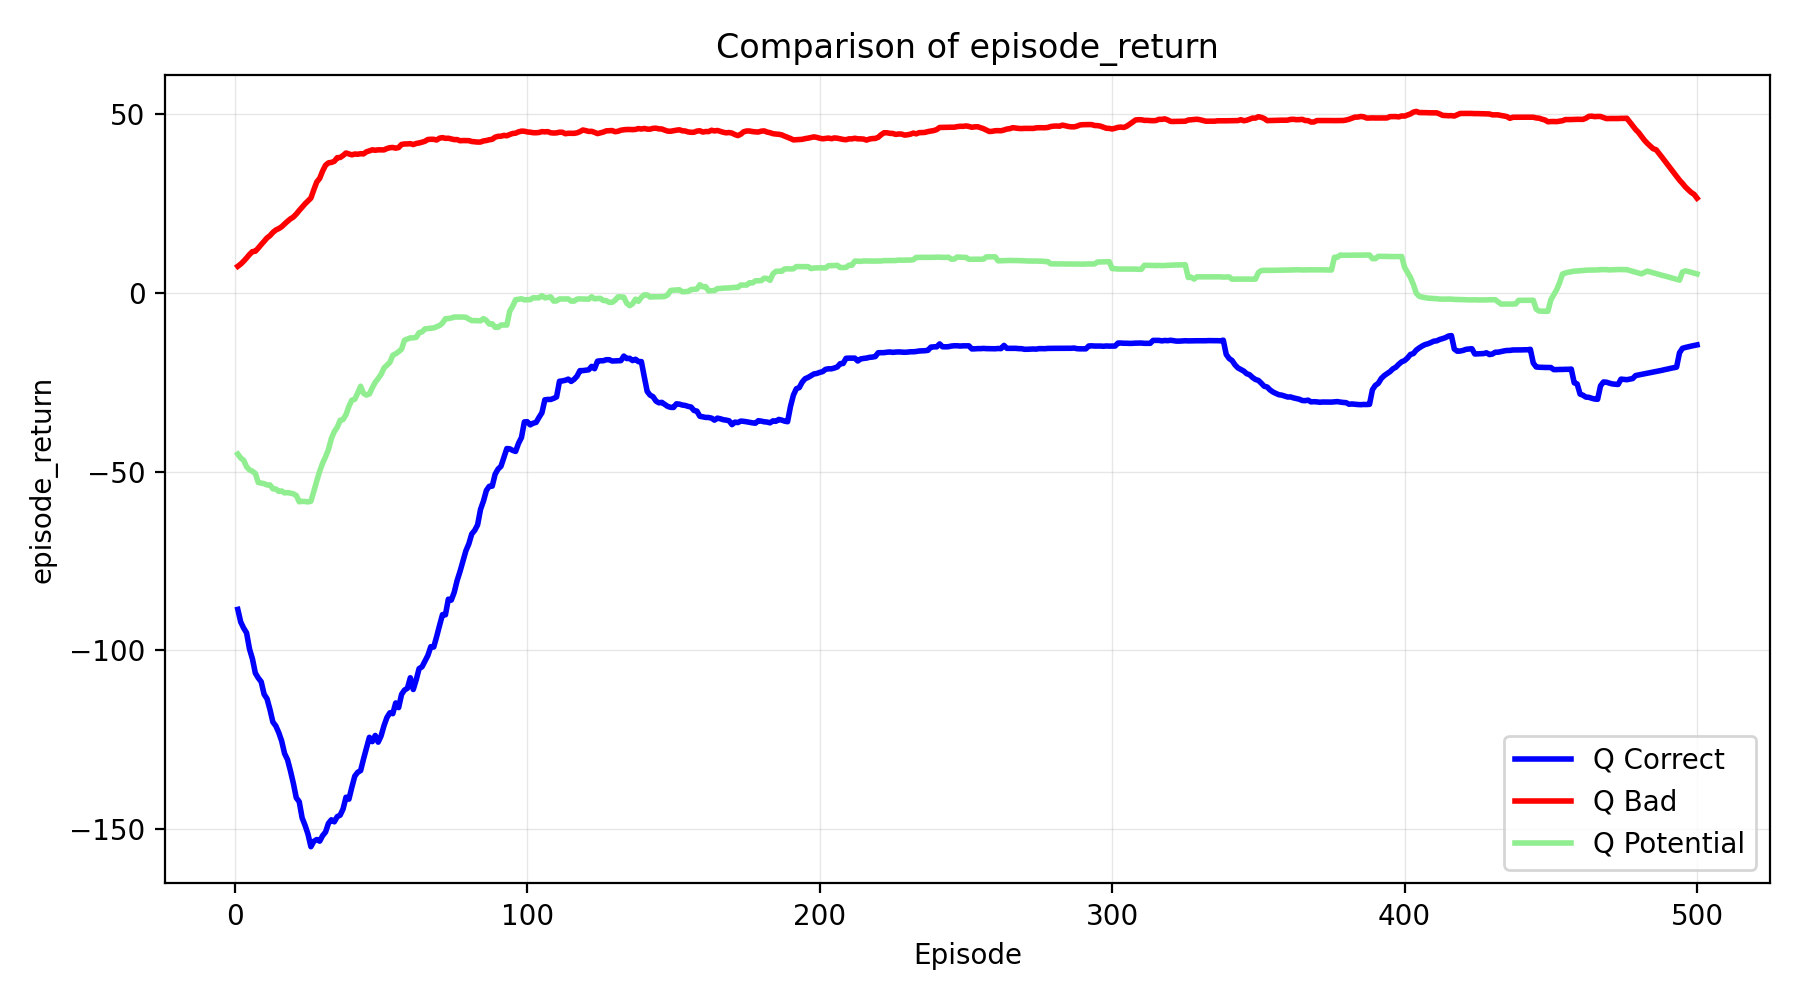
\includegraphics[width=0.47\linewidth]{./figures/plots/q_learning_return.png}
	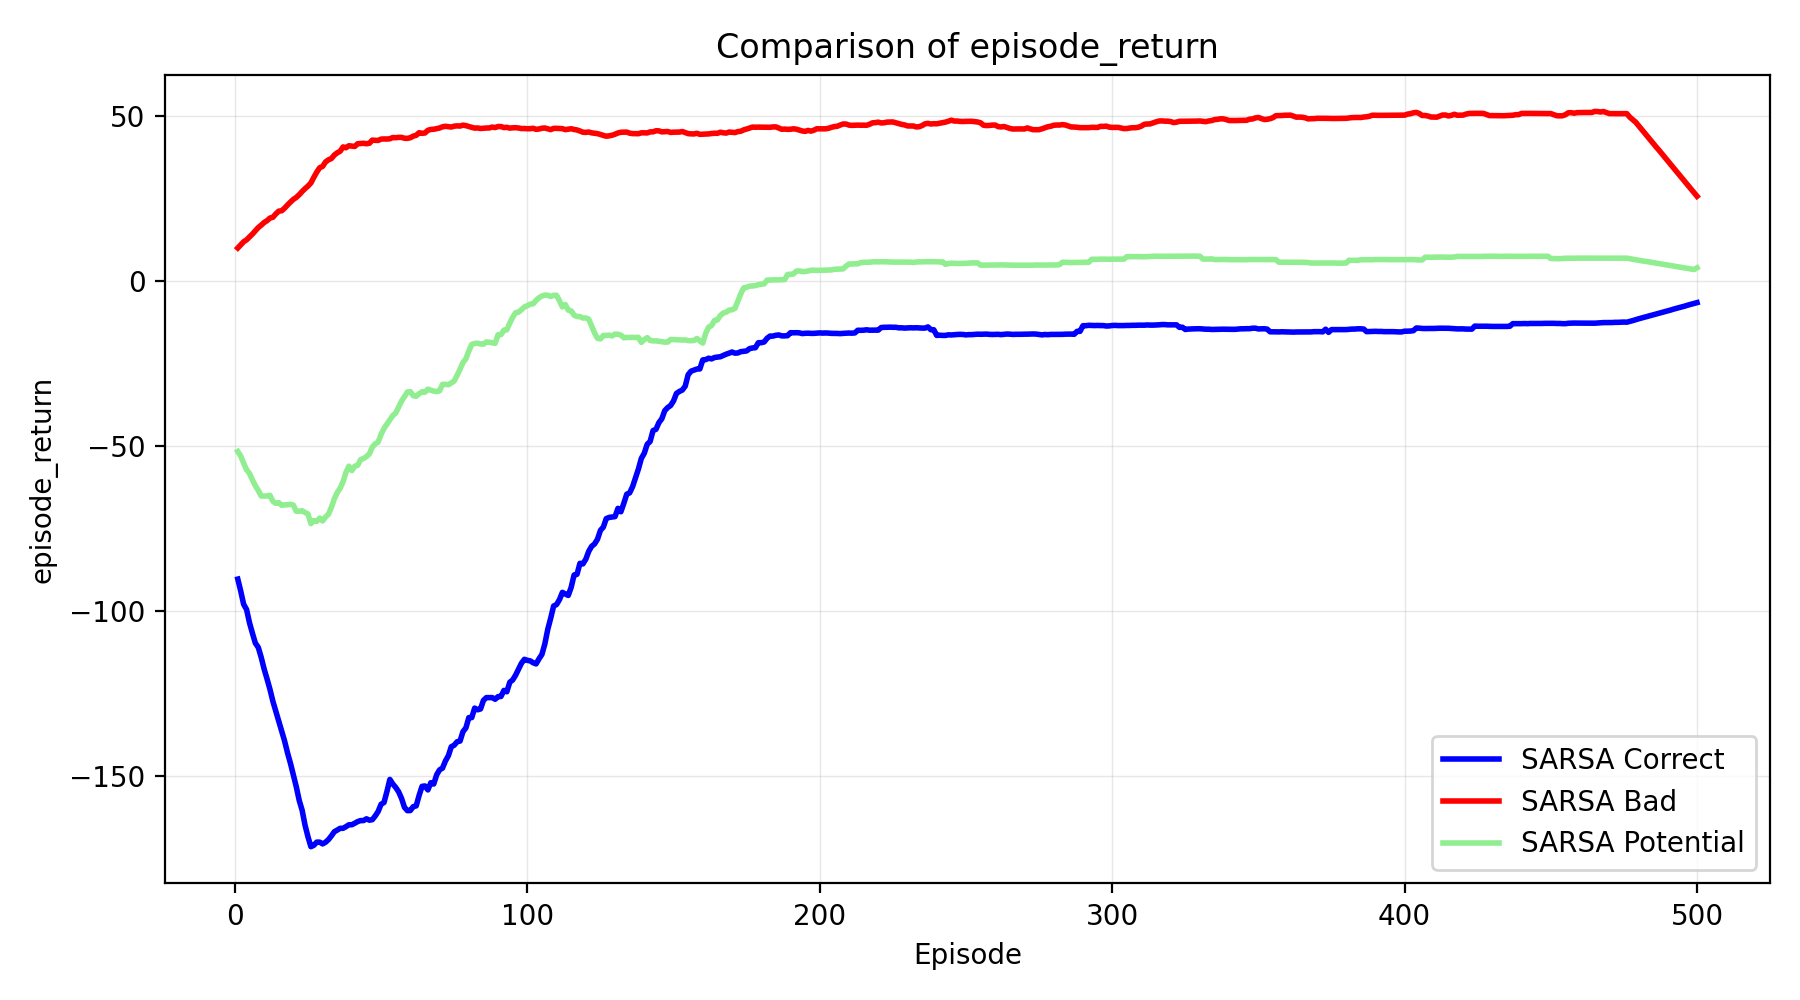
\includegraphics[width=0.47\linewidth]{./figures/plots/sarsa_return.png}
	\caption{Episode return for Q-learning (left) and SARSA (right) under the three reward settings.}
	\label{fig:returns}
\end{figure}

Figure~\ref{fig:returns} shows the learning curves for both algorithms. Under the correct reward, the returns improve steadily and eventually stabilize, indicating that both agents learn a sensible policy. Q-learning reaches high returns more quickly, which is consistent with its optimistic off-policy update rule. SARSA improves more gradually because it updates using the action actually taken under exploration and therefore incorporates the effect of stochasticity into learning.

The behavior under the misspecified reward is more interesting. In that case, Q-learning rapidly achieves high return, but this should not be interpreted as successful task completion. The return becomes high because the agent discovers a way to exploit the lure region. SARSA is also affected, but the effect is typically less abrupt, reflecting its more conservative update mechanism.

Under potential-based shaping, both algorithms improve significantly faster than under the correct reward. This is exactly the desired effect of shaping: the task is unchanged, but the reward signal becomes denser and therefore easier to learn from.

\begin{figure}[H]
	\centering
	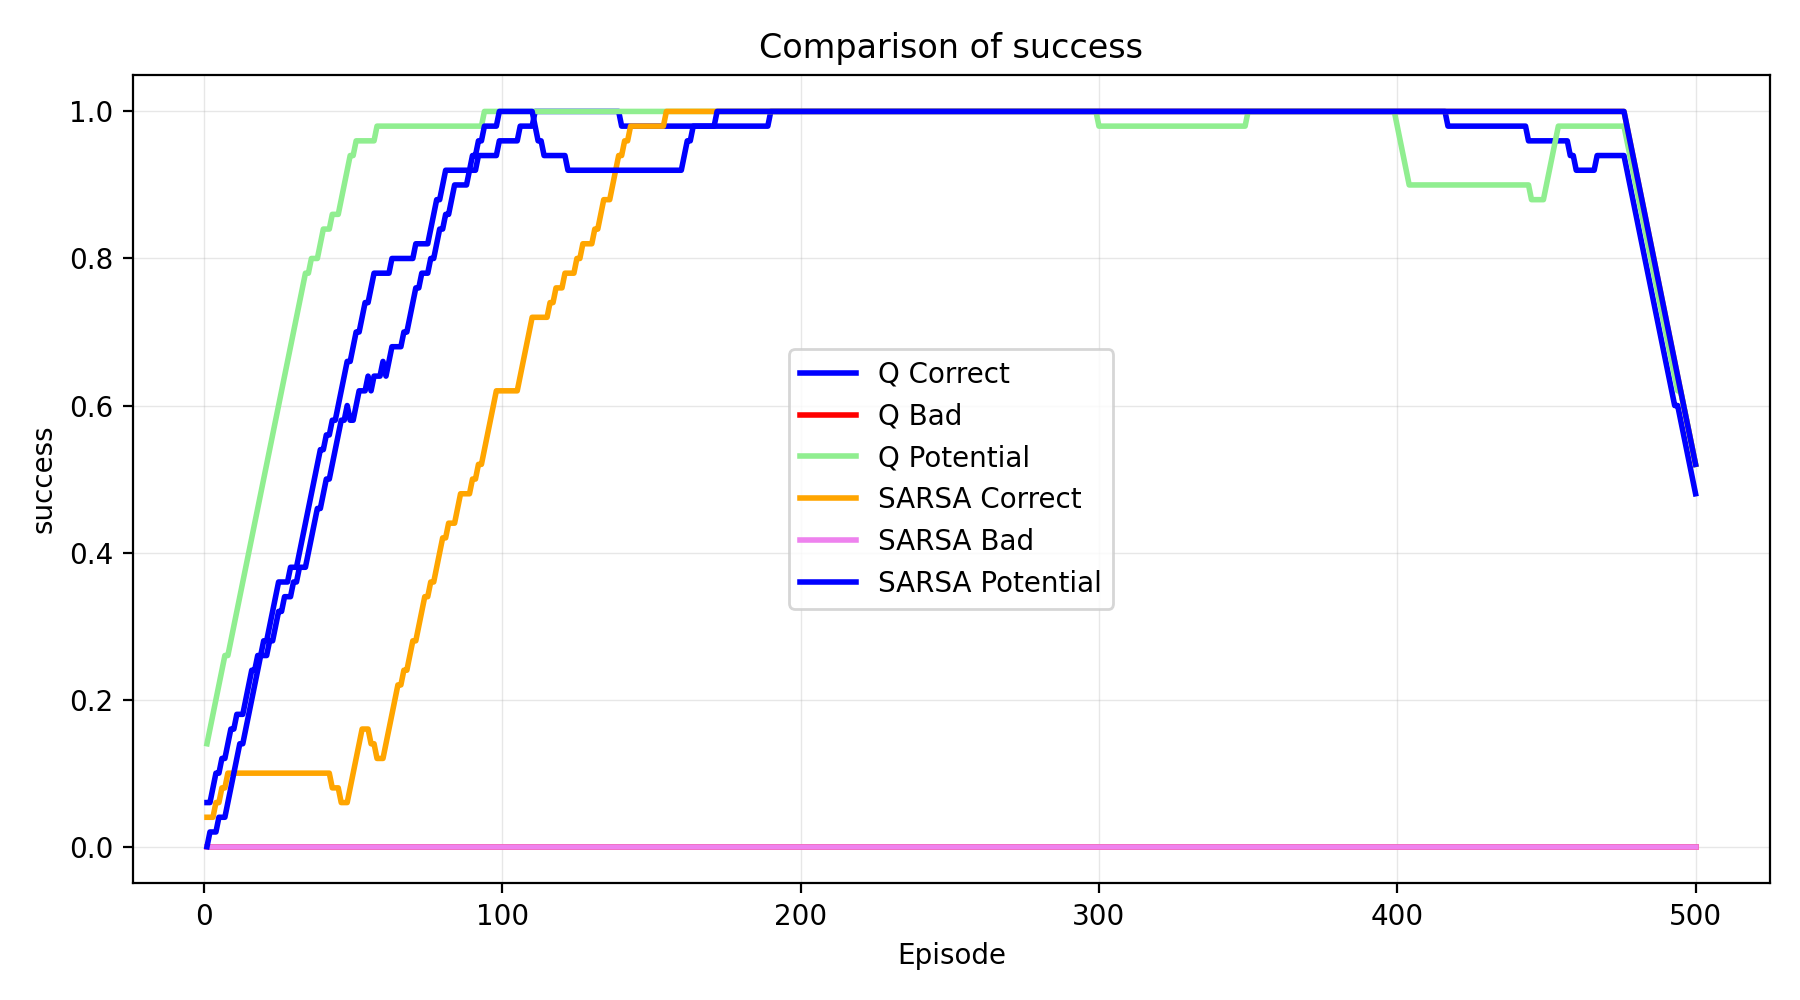
\includegraphics[width=0.68\linewidth]{./figures/plots/all_success.png}
	\caption{Success rate across training for all configurations.}
	\label{fig:success}
\end{figure}

The success rate in Figure~\ref{fig:success} complements the return curves and is arguably more informative. It shows that high return and actual task success may diverge sharply. In particular, the misspecified reward can produce large returns while the success rate remains poor, which is a direct signature of reward hacking. By contrast, the potential-shaped reward improves both return and success rate, confirming that it accelerates learning without biasing the goal.

\subsection{Value functions}

\begin{figure}[H]
	\centering
	
\includegraphics[width=0.32\linewidth]{./figures/q_learning_correct/figures/value_heatmap.png}
	
\includegraphics[width=0.32\linewidth]{./figures/q_learning_proximity_bad/figures/value_heatmap.png}
	
\includegraphics[width=0.32\linewidth]{./figures/q_learning_potential/figures/value_heatmap.png}

	\vspace{0.3cm}

	
\includegraphics[width=0.32\linewidth]{./figures/sarsa_correct/figures/value_heatmap.png}
	
\includegraphics[width=0.32\linewidth]{./figures/sarsa_proximity_bad/figures/value_heatmap.png}
	
\includegraphics[width=0.32\linewidth]{./figures/sarsa_potential/figures/value_heatmap.png}
	\caption{State-value heatmaps for all algorithm/reward combinations. Top row: Q-learning. Bottom row: SARSA. Columns: correct reward, misspecified reward, potential shaping.}
	\label{fig:values_all}
\end{figure}

The value heatmaps in Figure~\ref{fig:values_all} reveal how reward design modifies the internal structure learned by the agents. Under the correct reward, the value function forms a meaningful gradient toward the goal while reflecting the risk associated with the cliff. This is what one would expect from a well-aligned objective.

Under the misspecified reward, the value landscape becomes distorted. States near the lure region receive disproportionately high values because the agent expects to accumulate reward there. This distortion is not a learning failure in the algorithmic sense; rather, it is the logical consequence of optimizing a flawed objective. The agent is learning consistently with respect to the reward, but the reward itself is no longer aligned with the task.

Potential-based shaping yields value functions that remain globally consistent with the correct reward while being smoother and easier to propagate. This explains why learning is faster: the agent receives denser information about progress without changing which states are truly desirable in the long run.

Comparing Q-learning and SARSA also shows a qualitative difference. Q-learning often produces sharper value concentration, while SARSA tends to spread values more conservatively due to its on-policy nature and its sensitivity to noise.

\subsection{State visitation}

\begin{figure}[H]
	\centering
	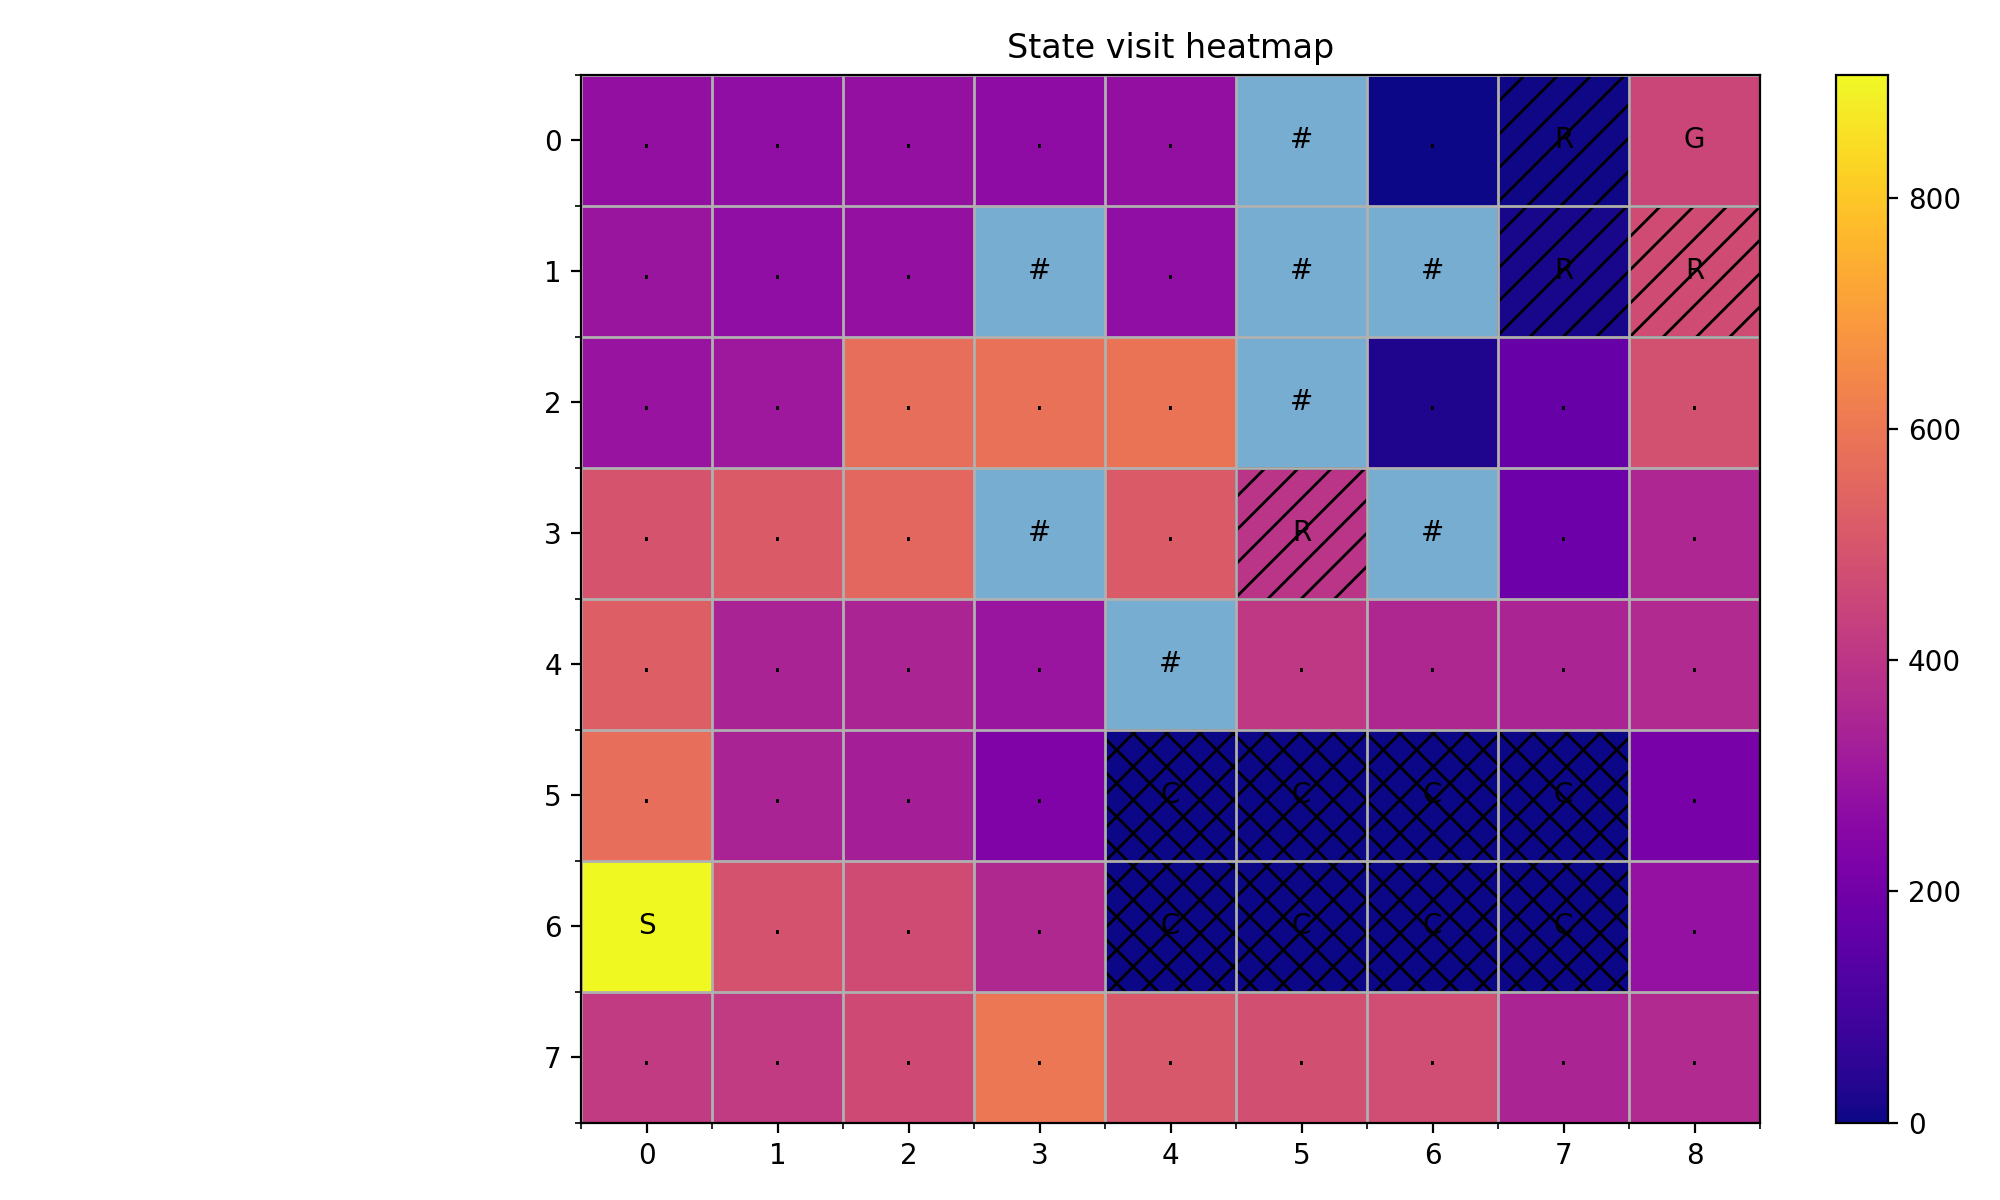
\includegraphics[width=0.32\linewidth]{./figures/q_learning_correct/figures/state_visits.png}
	
\includegraphics[width=0.32\linewidth]{./figures/q_learning_proximity_bad/figures/state_visits.png}
	
\includegraphics[width=0.32\linewidth]{./figures/q_learning_potential/figures/state_visits.png}

	\vspace{0.3cm}

	
\includegraphics[width=0.32\linewidth]{./figures/sarsa_correct/figures/state_visits.png}
	
\includegraphics[width=0.32\linewidth]{./figures/sarsa_proximity_bad/figures/state_visits.png}
	
\includegraphics[width=0.32\linewidth]{./figures/sarsa_potential/figures/state_visits.png}
	\caption{State visitation heatmaps for all algorithm/reward combinations. Top row: Q-learning. Bottom row: SARSA.}
	\label{fig:visits_all}
\end{figure}

State visitation frequencies in Figure~\ref{fig:visits_all} make the behavioral differences even more explicit. Under the correct reward, the agents progressively concentrate their visits along useful paths leading to the goal. Under potential shaping, this concentration appears earlier and more cleanly, which is consistent with faster convergence.

The misspecified reward produces a strikingly different pattern: visits accumulate in the lure region. This demonstrates that reward hacking is not merely a numerical effect in the return curve; it corresponds to a genuine reorganization of the agent’s behavior in space. The agent repeatedly returns to or remains near a locally rewarding area instead of solving the intended task.

Again, Q-learning tends to show a more concentrated exploitation of this region, while SARSA often exhibits a slightly more diffuse visitation pattern, reflecting its more cautious learning dynamics under stochastic transitions.

\subsection{Policies}

\begin{figure}[H]
	\centering
	
\includegraphics[width=0.32\linewidth]{./figures/q_learning_correct/figures/policy.png}
	
\includegraphics[width=0.32\linewidth]{./figures/q_learning_proximity_bad/figures/policy.png}
	
\includegraphics[width=0.32\linewidth]{./figures/q_learning_potential/figures/policy.png}

	\vspace{0.3cm}

	
\includegraphics[width=0.32\linewidth]{./figures/sarsa_correct/figures/policy.png}
	
\includegraphics[width=0.32\linewidth]{./figures/sarsa_proximity_bad/figures/policy.png}
	
\includegraphics[width=0.32\linewidth]{./figures/sarsa_potential/figures/policy.png}
	\caption{Greedy policies for all algorithm/reward combinations. Top row: Q-learning. Bottom row: SARSA.}
	\label{fig:policies_all}
\end{figure}

The policies in Figure~\ref{fig:policies_all} summarize the practical consequence of the reward formulations. Under the correct reward, both algorithms produce coherent goal-directed policies that avoid the most dangerous regions. SARSA’s policies are often slightly more conservative, especially near risk, which is consistent with its update rule.

Under the misspecified reward, the policy structure is altered in a systematic way. Instead of pointing reliably toward the goal, the arrows redirect the agent toward the lure region or induce local loops. This makes it visually clear that the learned policy is optimized for the wrong objective.

Potential-based shaping restores a policy close to that obtained with the correct reward, but usually with cleaner structure and earlier convergence. This is one of the strongest experimental confirmations in the report: not all dense rewards are problematic, only those that alter the optimization target.

\subsection{Trajectories}

\begin{figure}[H]
	\centering
	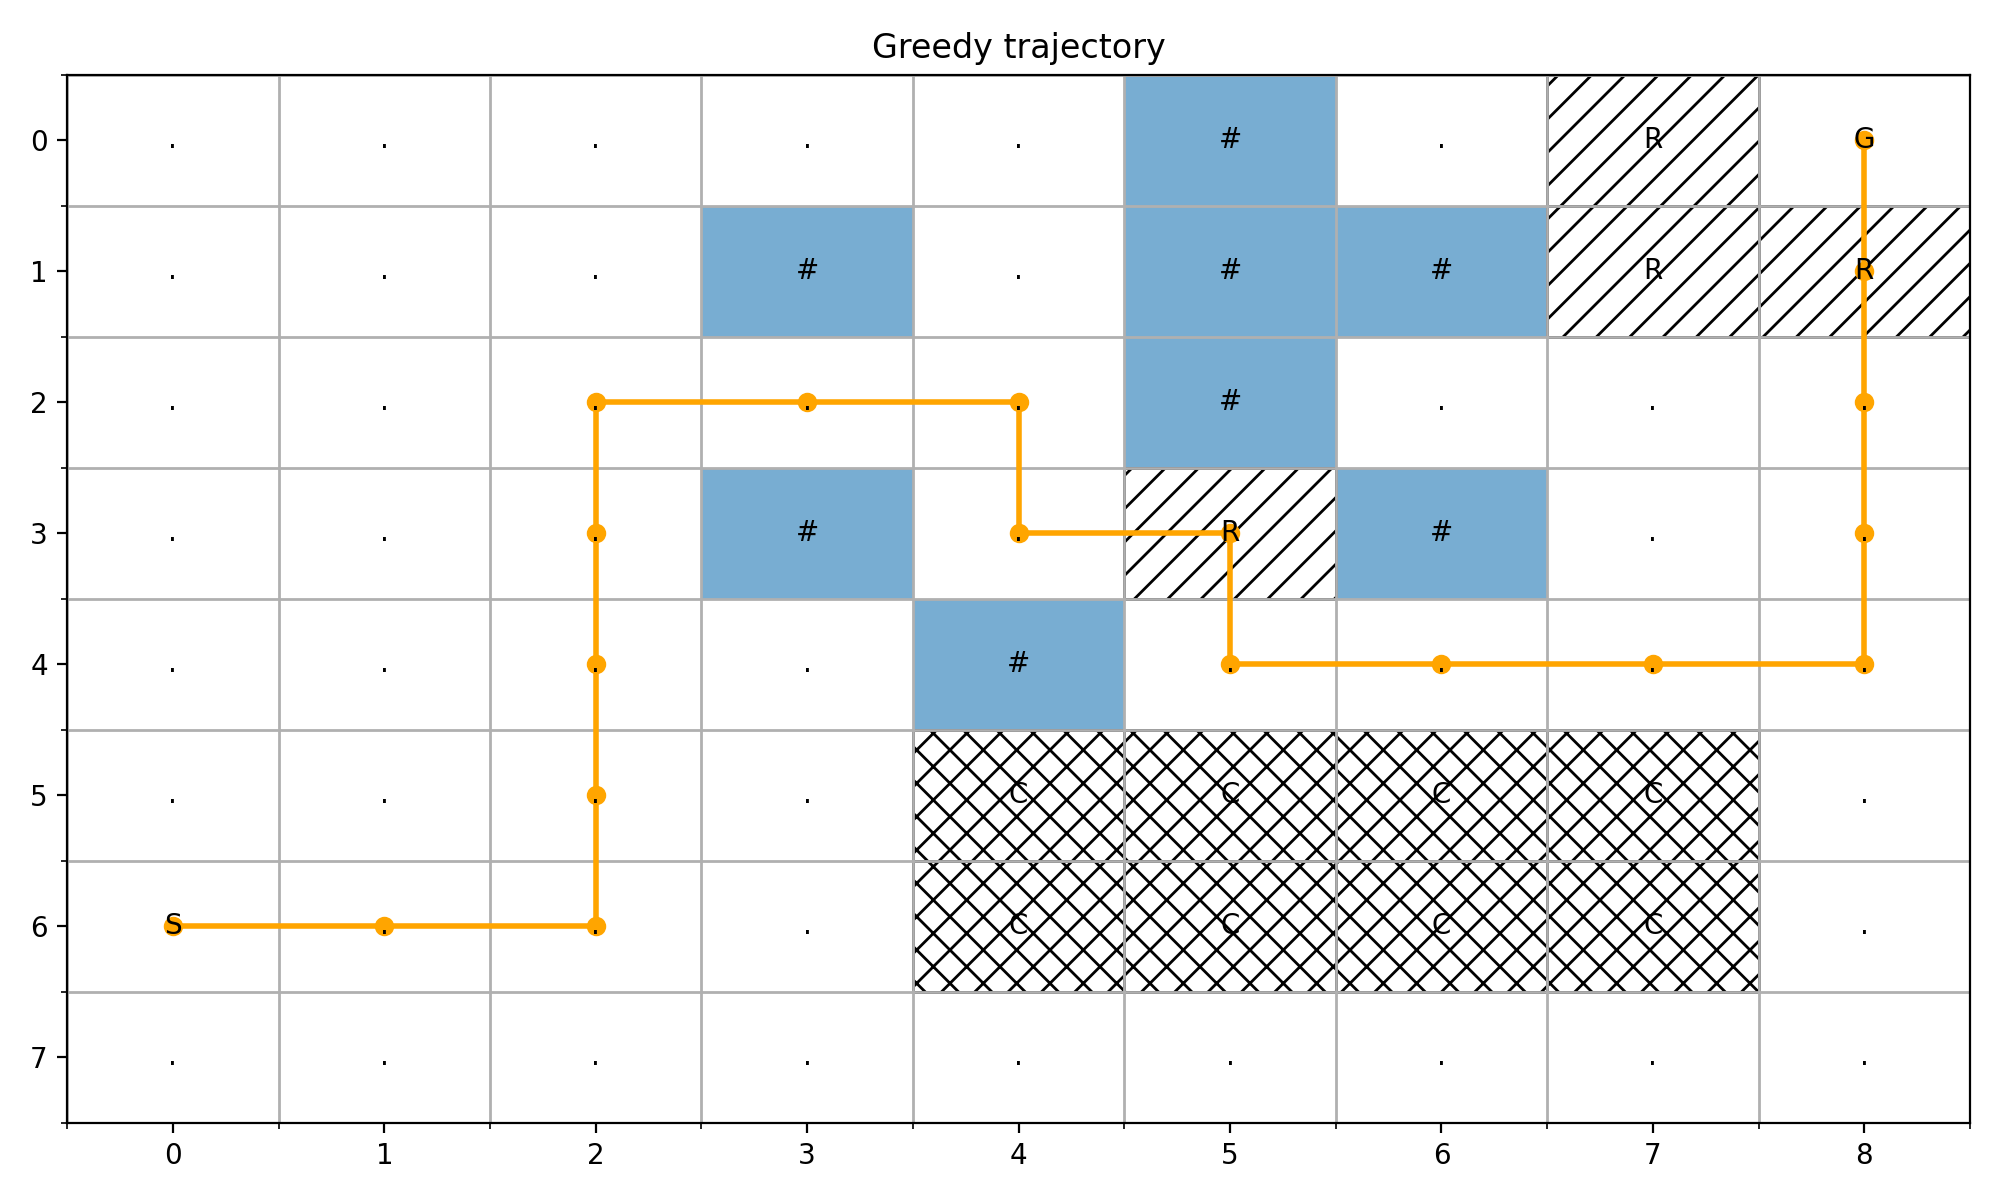
\includegraphics[width=0.32\linewidth]{./figures/q_learning_correct/figures/greedy_trajectory.png}
	
\includegraphics[width=0.32\linewidth]{./figures/q_learning_proximity_bad/figures/greedy_trajectory.png}
	
\includegraphics[width=0.32\linewidth]{./figures/q_learning_potential/figures/greedy_trajectory.png}

	\vspace{0.3cm}

	
\includegraphics[width=0.32\linewidth]{./figures/sarsa_correct/figures/greedy_trajectory.png}
	
\includegraphics[width=0.32\linewidth]{./figures/sarsa_proximity_bad/figures/greedy_trajectory.png}
	
\includegraphics[width=0.32\linewidth]{./figures/sarsa_potential/figures/greedy_trajectory.png}
	\caption{Greedy trajectories for all algorithm/reward combinations. Top row: Q-learning. Bottom row: SARSA.}
	\label{fig:traj_all}
\end{figure}

The greedy trajectories in Figure~\ref{fig:traj_all} provide the most direct behavioral evidence. Under the correct reward, the agent typically reaches the goal by following a reasonable path. Under misspecified reward, the trajectory often becomes trapped in the lure region, confirming that the learned policy is not simply noisy or unstable, but systematically redirected by the reward structure. Under potential shaping, the greedy trajectory remains efficient and goal-directed.

These trajectories make it possible to distinguish clearly between three cases:
\begin{itemize}
	\item correct reward: slower but valid learning,
	\item misspecified reward: high return but incorrect behavior,
	\item potential shaping: faster learning with preserved task objective.
\end{itemize}

\section{Conclusion}

This study shows that reward design plays a central role in reinforcement learning, often as important as the learning algorithm itself. Misspecified rewards do not merely slow down learning; they can fundamentally redirect it, leading agents to develop behaviors that are perfectly rational with respect to the reward signal but completely misaligned with the intended goal. This is the essence of reward hacking.

At the same time, the results also show that shaping is not inherently problematic. Potential-based shaping provides a principled way to densify the reward signal while preserving the optimal policy, leading to substantial gains in learning speed and robustness.

Finally, comparing Q-learning and SARSA illustrates that algorithmic differences remain relevant, especially in noisy environments. Q-learning is faster and more aggressive, but also more sensitive to reward bias. SARSA is slower yet more conservative and robust. Still, across all experiments, the dominant factor remains the reward formulation itself.

\end{document}
